\documentclass{article}
\usepackage{setspace}
\usepackage[round]{natbib}   % omit 'round' option if you prefer square brackets
%\usepackage{natbib}
\bibliographystyle{abbrvnat}
\usepackage[utf8]{inputenc}
\usepackage[T1]{fontenc}

\usepackage{mathtools}% Loads amsmath
\usepackage[utf8]{inputenc}
\usepackage{lmodern}
\usepackage[a4paper, margin=1in]{geometry}
\usepackage{amsmath,amsthm,amssymb}
\usepackage[titletoc]{appendix}
\usepackage{esint}
\usepackage{graphicx}
\usepackage{listings}
\usepackage{threeparttable}
\usepackage[referable]{threeparttablex}
\usepackage{booktabs, longtable}
\newcounter{tablenote}[table]
\newcommand{\itemx}[1]{
    \stepcounter{tablenote}
    \item[\thetablenote]\label{#1}
}

\usepackage{xspace,color}
\usepackage{url}
\usepackage{listings}
\usepackage{newpxtext,newpxmath}
\lstset{commentstyle=\color{red},keywordstyle=\color{black},
showstringspaces=false}
\lstnewenvironment{rc}[1][]{\lstset{language=R}}{}
\newcommand{\ri}[1]{\lstinline{#1}}  %% Short for 'R inline'
\lstset{language=R}             % Set R to default language

\usepackage{footnote}
\usepackage{hyperref}
\usepackage{tablefootnote}
\usepackage{lipsum}
\usepackage{minted}
\usepackage{bm}
\usepackage{mathtools}
\usepackage{footnote}
\usepackage{nccmath}
\usepackage{breqn}
\usepackage{empheq}
\usepackage{booktabs}
\usepackage{array}
\usepackage{chngcntr}
\counterwithin{table}{section}
\usepackage{xcolor}
\definecolor{shadecolor}{RGB}{220,220,220}
\newcommand{\mybox}[1]{\par\noindent\colorbox{shadecolor}
{\parbox{\dimexpr\textwidth-2\fboxsep\relax}{#1}}}
\counterwithin{figure}{section}
\usepackage{multirow}
\makeatletter
\newcommand{\distas}[1]{\mathbin{\overset{#1}{\kern\z@\sim}}}%
\newsavebox{\mybox}\newsavebox{\mysim}
\newcommand{\distras}[1]{%
  \savebox{\mybox}{\hbox{\kern3pt$\scriptstyle#1$\kern3pt}}%
  \savebox{\mysim}{\hbox{$\sim$}}%
  \mathbin{\overset{#1}{\kern\z@\resizebox{\wd\mybox}{\ht\mysim}{$\sim$}}}%
}
\makeatother
\numberwithin{equation}{section}
\large

\onehalfspacing
\theoremstyle{plain}

\newtheorem*{theorem*}{Theorem}
\newtheorem{theorem}{Theorem}
\begin{document}

\begin{onehalfspacing}
\begin{titlepage}			%makes a title page. Remember to change the author, CID, username and group number to what is appropriate for you!
	\centering
	{\scshape\LARGE University of British Columbia\par}
	{\scshape \LARGE Department of Statistics\par}
	\vspace{1cm}
	{\LARGE \bfseries Some Thoughts about Prior Distribution and Sample Size in Bayesian Modeling\par}
 % {\LARGE \bfseries \textit{Some Thoughts about Prior Distribution and Sample Size}\par}
	\vspace{1cm}
	{\Large \bfseries STAT 536D Final Assignment\par}
	\vspace{3cm}
	{\Large\itshape Qian Ye \par}		%remember to change these!
	\vspace{0.5cm}
	%		{\large Group \@group\unskip\strut\par}
	{\large \itshape 15780109\par}		%remember to change these!
	\vspace{1cm}
	{\large \today\par}
\end{titlepage}
\end{onehalfspacing}

\section{Introduction}
For likelihood-based inference, the likelihood function of observed data contains all the information available about the unknown parameter: The maximum likelihood estimate (MLE) can be obtained by maximizing the likelihood function and its variance can be calculated from the Fisher information, which is the negative second derivative of the log-likelihood function. Whereas, the posterior distribution forms the basis of Bayesian inference and contains all the formation about the parameter. The Bayesian inference is entirely derived from characteristics of the posterior distribution. For example, the posterior mean can be used as the Bayesian point estimate and the posterior quantiles can be used as bounds for a credible interval. Thus, by looking into the posterior distribution, we can get more insights about Bayesian inference. Considering the posterior distribution is determined by the prior distribution and likelihood function of the observed data, I focus my investigation on the relation between the prior distribution and the observed data, particularly the size of the observed samples, in this report. 

\section{Prior and Sample Size}
\label{sec:prior}
Firstly I introduce the notations. Let $\theta$ denote the unknown parameter of interest with a prior distribution $p(\theta)$, $X_{1:n}=\{X_i,i=1,\cdots,n\}$ denote a random sample from a distribution $f(x|\theta)$ and $x_{1:n}=\{x_i,i=1,\cdots,n\}$ denote its observed realization. Then, we can compute the density function $f(\theta|x_{1:n})$ of the posterior distribution using Bayes’ theorem
\begin{align}\label{eq:bayes}
    \underbrace{f(\theta|x_{1:n})}_{\text{posterior}} =
    \frac{p(\theta)\prod^n_{i=1}f(x_i|\theta)}{\int p(\theta)\prod^n_{i=1}f(x_i|\theta)\,\mathrm{d}\,\theta} \propto \underbrace{p(\theta)}_{\text{prior}}
    \underbrace{\prod^n_{i=1}f(x_i|\theta)}_{\text{likelihood: }L(\theta|x_{1:n})}.
\end{align}

The equation \eqref{eq:bayes} is the essential in Bayesian inference, from which we can intuitively observe that
\begin{itemize}
    \item the only additional information contained by the posterior distribution compared to the likelihood function is the information given by the prior distribution;
    \item The posterior distribution becomes more heavily impacted by the likelihood as the sample size increase, because the information contained by likelihood $L(\theta|x_{1:n})$ increases as the sample size increases but the information contained by the prior stays fixed.
\end{itemize}
The first observation may inspire a fundamental question in Bayesian analysis that how much the posterior inference would be influenced by the additional information contained in the prior. While the second observation partially answers it: when sample size is large enough, the information in the posterior distribution is denominated by the likelihood of observed data and information contained in the prior may be neglected, and therefore, the Bayesian inference based on the posterior distribution would potentially yield similar results as the likelihood inference, regardless of information in the prior. To formally fix the idea, I briefly introduce the asymptotic normality of the posterior distribution:
\begin{theorem}[Asymptotic normality of the posterior distribution]\label{th:asy}
Any posterior distribution is (under suitable regularity conditions) asymptotically normal with mean equal to the MLE and covariance equal to the inverse observed Fisher information matrix:
$$
\theta|x_{1:n} \rightarrow_d \mathcal{N}\left(\hat{\theta}_{mle}, I^{-1}(\hat{\theta}_{mle})\right).
$$
\end{theorem}

Now we have known that the Bayesian estimate, e.g.\ the posterior mean, converges to the MLE in distribution with infinite sample size, neglecting the prior. If you are looking for more technical details about the theorem, \cite{Held2014} would be a good reference. Nevertheless, in the case of small or moderate sample size Bayesian inference results can be subtle, as the second observation implies that the information contained in the prior distribution plays a much larger role in the Bayesian inference with a limited sample size. Consequently, the amount of information contained in the prior is of special importance when applying Bayesian analysis in settings with a small to moderate sample size. For instance, when fitting a Bayesian model to a data set with a few observations (e.g.\ n=10), a very informative prior, rather than the observed data, tends to dominate posterior inferences. In this situation, an informative prior elicited from an expert is appealing, with which the Bayesian model may still provide relatively valid inference, because the valid information in the prior would compensate the lack of observed data. On the contrary, the prior is often chosen for a technically convenient in practice, then we need to consider the prior choice with more caution, as an improper prior may inappropriately introduce artificial information, thus leading to invalid inference. In a word, a ``good'' prior potentially allows the Bayesian model to achieve valid inference with a very loose requirement on sample size, whereas a ``bad'' one may lead to invalid posterior inference without enough number of observations. To better illustrate the relation of prior and sample size, I demonstrate a simple example in next section. 
  
\section{A Simple Example}
\label{sec:example}
Suppose we conduct inference for a proportion based on a random sample of size $n$ with $Y=y$ of individuals in this sample succeeding in a certain event of interest. We reasonably assume a binomial model with the unknown probability $\pi \in (0,1)$ to the random variable $Y$, i.e.\ $Y \sim \mathrm{Bin}(n, \pi)$. A beta prior distribution is often assumed for the parameter $\pi$, that is \ $\pi \sim \mathrm{Beta}(\alpha, \beta)$, where $\alpha,\beta>0$, since the beta distribution is conjugate prior for the binomial likelihood. Then, we have 
\begin{align*}
    p(\pi)&=\frac{1}{\mathrm{B}(\alpha, \beta)}\pi^{\alpha-1}(1-\pi)^{\beta-1},\\
    L(\pi|y)&=f(y|\pi)=C^y_n\pi^y(1-\pi)^{n-y},
\end{align*}
and thus the posterior distribution can be computed as
\begin{align*}
    f(\pi|y) & \propto p(\pi)L(\pi|y)\\
    &\propto \pi^{\alpha-1}(1-\pi)^{\beta-1} \times \pi^y(1-\pi)^{n-y} \\
          &   = \pi^{\alpha+y-1}(1-\pi)^{\beta+n-y-1},
\end{align*}
which identifies another beta distribution with parameters $\alpha+y$ and $\beta+n-y$:
\begin{align*}
    \pi|y \sim \mathrm{Beta}(\alpha+y, \beta+n-y).
\end{align*}
The logic underlying the Bayesian inference in this example is that, after having observed the data $(n,y)$, the distribution of the parameter $\pi$ is updated to $\mathrm{Beta}(\alpha+y, \beta+n-y)$ from the prior $\mathrm{Beta}(\alpha, \beta)$. Namely, the point estimate of $\pi$ is updated to the posterior mean $\mu_{n}=(\alpha+y)/(\alpha+\beta+n)$ from the prior mean $\mu_{0}=\alpha/(\alpha+\beta)$. Let's re-write the the posterior mean as
\begin{align}\label{eq:pomean}
    \mu_{n}=\frac{\alpha+y}{\alpha+\beta+n}
=\frac{\alpha+\beta}{\alpha+\beta+n}\cdot \frac{\alpha}{\alpha+\beta}+
\frac{n}{\alpha+\beta+n}\cdot \frac{y}{n}.
\end{align}

We can think of the prior distribution $\mathrm{Beta}(\alpha, \beta)$ as if $\alpha$ successes were already observed in $\alpha+\beta$ trials before the random sample of size $n$ is actually obtained. Hence, the sum of $\alpha+\beta$ can be treated as a \textit{prior sample size}, denoted by $n_0$. The value of $y/n$ is actually the MLE of $\pi$, denoted by $\hat{\pi}_{mle}$. So, Equation \eqref{eq:pomean} can be written as
\begin{align}\label{eq:wtmean}
    \mu_n=\frac{n_0}{n_0+n}\cdot\mu_0+\frac{n}{n_0+n}\cdot \hat{\pi}_{mle},
\end{align}
which shows that the posterior mean is a weighted average of the prior mean and the MLE, with weights proportional to the prior sample size $n_0$ and the data sample size $n$, respectively. 

As the data sample size $n$ increases, the weight of the prior mean decreases and the posterior mean $\mu_n$ will come closer to $\hat{\pi}_{mle}$. Eventually, when $n \rightarrow \infty$, the weight of the prior mean is approaching to zero and the posterior mean $\mu_n$ converges to $\hat{\pi}_{mle}$, which is a manifestation of Theorem \ref{th:asy}. However, in settings with a small to moderate sample size $n$, the prior mean $\mu_0$ will influence the posterior mean $\mu_n$ and the extent of the influence is determined by its weight $n_0/(n_0+n)$. Going back to the instance where one fits a Bayesian model to a data set with $n=10$, an informative prior with $n_0=10$ or more dominates posterior inference, and consequently the prior mean determines the accuracy of the posterior estimate. 

For more complex Bayesian models, unfortunately, we no longer always have an analytic expression for the posterior mean as shown in Equation \eqref{eq:wtmean}. To further demonstrate the relation between the prior and sample size under a more complicated model, I conduct a simulation study in the later section to empirically show the impact of the prior on the Bayesian inference in various settings of sample size. 

\section{A Simulation Study}
\label{sec:sim}
\subsubsection*{\textit{Data generation}}
I borrow the data generation mechanism from Lecture 2: a binary outcome $Y \in \{0,1\}$ with two binary risks factor $(X_1, X_2)$ is considered, with the underlying relationship given by a logistic regression model, written as
\begin{align}\label{eq:logis}
    \mathrm{logit}(P(Y=1))=\beta_0+\beta_1X_2+\beta_2X_2,
\end{align}
where the true parameter values are set to be $(\beta_0, \beta_1, \beta_2)=(-1,0.2, 0.6)$. The risk factors $(X_1, X_2)$ are generated from two Bernoulli distribution, that is, $X_1\sim \mathrm{Bern}(0.4)$ and $X_2\sim \mathrm{Bern}(0.2+0.5X_1)$. Bayesian inference is employed to provide point estimates and standard errors for all parameters in model \eqref{eq:logis}, however, the results for one parameter, $\beta_2$, are in focus here for illustrative convenience. 

\subsubsection*{\textit{Settings of prior and sample size}}
I choose a very flat distribution $\mathcal{N}(0, 10^2)$ to be the vague or non-informative prior for $\beta_0$ and $\beta_1$, while take into account different prior distributions for $\beta_2$ to reflect different levels of prior informativeness that are put into the Bayesian inference. Specifically, we consider
\begin{itemize}
    \item Prior 1: $\beta_2 \sim \mathcal{N}(0, 10^2)$; non-informative prior,
    \item Prior 2: $\beta_2 \sim \mathcal{N}(0.6, 2^2)$; very informative prior centered at 0.6,
    \item Prior 3: $\beta_2 \sim \mathcal{N}(0, 2^2)$; very informative prior centered at 0,
    \item Prior 4: $\beta_2 \sim \mathcal{N}(-0.6, 2^2)$; very informative prior centered at -0.6.
\end{itemize}
When looking at the informative Prior 2, 3, and 4, successively, the location of the center of the prior distribution is getting further away from the true value $\beta_2=0.6$, which implies the Bayesian inference may become more heavily impacted by the inappropriate artificial information. A variety settings of sample size are considered, that is, $n=10,20,40,50,100, 500,$ and $1000$. 

\subsubsection*{\textit{Results}}
For each setting of prior and sample size, I run 500 simulation replicates for the model and obtain 500 posterior means as estimates of $\beta_2$. Then, the empirical mean and standard deviation of the 500 estimates are reported in Figure \ref{fig:estimate} to evaluate the performance of Bayesian inference. In the figure, the solid points indicate the empirical means and the horizontal error bars represent one (empirical) standard deviation of uncertainty, i.e.\ mean $\pm$ standard deviation. Note that the MLEs of $\beta_2$ based on classical likelihood inference are also included for comparison. All simulation and analysis code used in this study are available on GitHub (\url{https://github.com/QianYe-stat/STAT536D-Final}).
\begin{figure}[H]
    \centering
    \caption{MLE and Bayesian estimates with various prior distributions, in different settings of sample size; the true value of the parameter is $\beta_2=0.6$}
    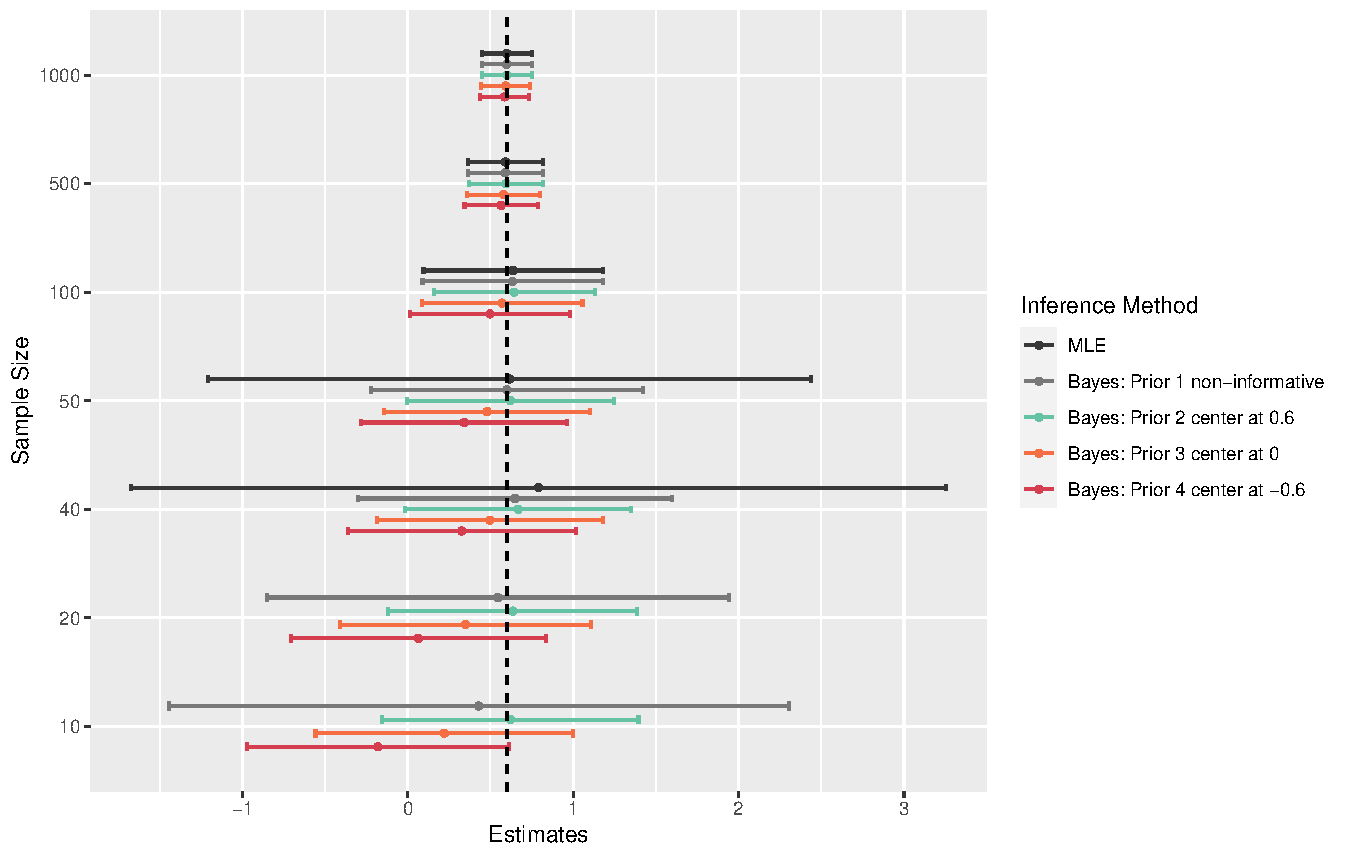
\includegraphics[scale=0.75]{figures/Estimates.pdf}
    \label{fig:estimate}
    \begin{minipage}{\textwidth} 
{\footnotesize Note: the dashed vertical line indicates a reference representing the true parameter value of 0.6. The MLEs for sample size 10 and 20 are omitted in the figure for a better presentation, as the associated empirical standard deviations are substantially larger compared to those from other settings. The figure showing complete estimation from all settings can be seen in Appendix \ref{app:suppfig}.\par}
\end{minipage}
\end{figure}
Firstly, we see that the Bayesian estimates, no matter which prior distribution is used, seem to come fairly close to the MLEs for increasing sample size. When the sample size is large enough, e.g.\ n=1000 in this study, all Bayesian estimates are almost identical to the MLE, regardless of the priors. This result can be viewed as an empirical demonstration of Theorem \ref{th:asy}. 

Secondly, it can be observed that an informative prior distribution heavily impacts the posterior distribution when applying Bayesian model in settings with a small to moderate sample size. When sample sizes are 10 to 50, Prior 4 consistently leads to the most biased posterior estimates among the four Bayesian models, which is not surprising, as the location of the center of Prior 4 deviates the most from the true parameter value. On the contrary, Prior 2, which is centered at the true parameter value, always produces accurate posterior estimates for the parameter, even though the sample size is very limited, e.g.\ $n=10$. This observation again confirms what we have observed in the example in Section \ref{sec:example} that a ``good'' prior potentially allows the Bayesian methods to provide valid inference with a very loose requirement on sample size, whereas a ``bad'' prior may lead to invalid posterior inference without enough number of observations.

Thirdly, we find that the Bayesian inference is much more efficient than the likelihood inference when the sample size is small or moderate. In the case that the sample size is 50 or less, the standard deviations of Bayesian estimates are much smaller compared to those of corresponding MLEs. This may imply that the Bayesian inference, even with a non-informative prior, requires less observed samples to achieve the same level of efficiency as the likelihood inference. 

Last but not the least, the performance of Bayesian inference with a non-informative prior surprises me the most. Even with a very limited sample size, e.g,\ n=10 or 20 in this study, it still can provide satisfactory estimates with acceptable efficiency, especially when compared with the likelihood inference results (see Figure \ref{fig:estimate_full}). Therefore, when we don't have confidence about the validity of the prior information or purely avoid introducing artificial information, a vague or non-informative prior is strongly recommended. 

\section{Further Reading}
There are some further readings if you are interest. From the example in Section \ref{sec:example}, we see that the prior sample size is a very good index to evaluate a prior's informativeness, and the computation of prior sample size seems straightforward in that particular example. For many parametric Bayesian models, however, it is not obvious how to determine the sample size of the prior. \cite{Morita2008} presents a definition for the effective sample size of a parametric prior distribution in a Bayesian model, and propose methods for computing the effective sample size in a variety of settings. In addition, \cite{Sahu2006} propose innovative simulation-based techniques of sample size determination within the Bayesian framework. One of their key results is that typical non-informative prior distributions lead to very small sample sizes. In contrast, a very informative prior distribution may either lead to a very small or a very large sample size depending on the location of the centre of the prior distribution and the hypothesized value of the parameter. This finding inherently agrees what we have discussed in Section \ref{sec:prior}, and is manifested by the simulation results shown in Section \ref{sec:sim}.
 
\bibliography{bibtex}

\newpage
\appendix
\section{Supplementary Figure for the Simulation Study}
\label{app:suppfig}
\begin{figure}[H]
    \centering
    \caption{Parameter estimation from various inference methods}
    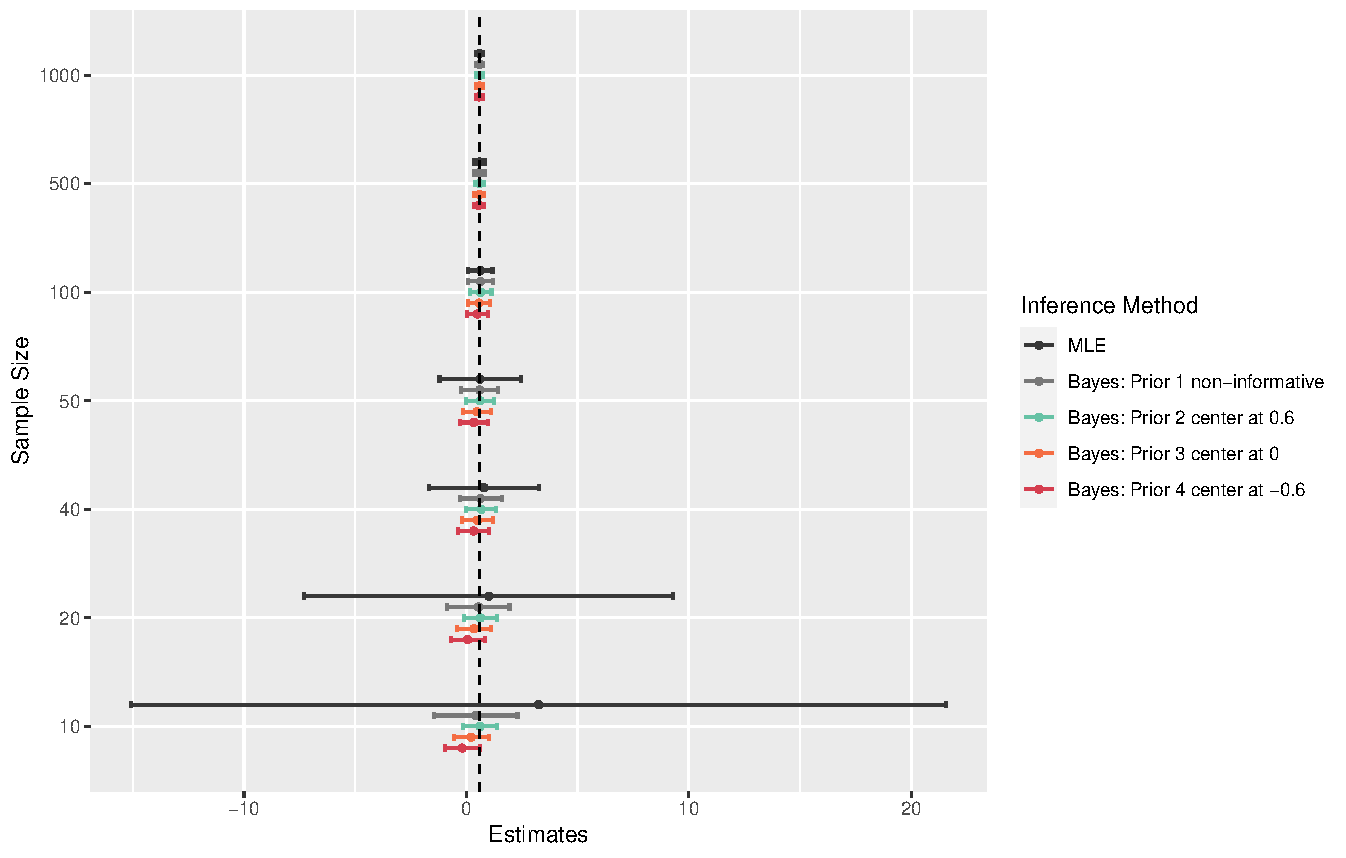
\includegraphics[scale=0.7]{figures/Estimates_full.pdf}
    \label{fig:estimate_full}
\end{figure}
 

\end{document}













